\documentclass[10pt, a4paper]{article}

% On écrit en français
\usepackage[utf8]{inputenc}
\usepackage[frenchb]{babel}
\usepackage[T1]{fontenc}

% Packages nécessaires
\usepackage{graphicx}
\usepackage{hyperref}

% Numérotation de page custom
\usepackage{fancyhdr}
\usepackage{lastpage}
\pagestyle{fancy}
\fancyhf{}
\rfoot{Page \thepage \hspace{1pt} sur \pageref{LastPage}}

% Police Helvetica <3
\usepackage{helvet}
\renewcommand*{\familydefault}{\sfdefault}

% Enlever les alinéas
\setlength{\parindent}{0pt}

% Marges plus larges pour faire moins LaTeX
\usepackage[left=3cm, right=3cm]{geometry}

% Sous titre de document
\usepackage{titling}
\newcommand{\subtitle}[1]{%
  \posttitle{%
    \par\end{center}
    \begin{center}\large#1\end{center}
    \vskip0.5em}%
}

% En tête complet de document
\newcommand{\Document}[1]{%
    \title{#1}
    \subtitle{Dématérialisation d'un processus de paiement}
    \author{
        COMETS Jean-Marie \\
        DELMARRE Adrian \\
        REYNOLDS Nicolas \\
        TURPIN Pierre
    }
    \date{\today}

    \maketitle \newpage

    \tableofcontents \newpage
}


\begin{document}

\Document{Architecture technique}

\section{Présentation générale}

La figure \ref{fig:network} détaille l'architecture technique choisie.
Cependant, certains points doivent être justifiés ou davantage expliqués.

\begin{landscape}
  \begin{figure}[htpb]
      \centering
      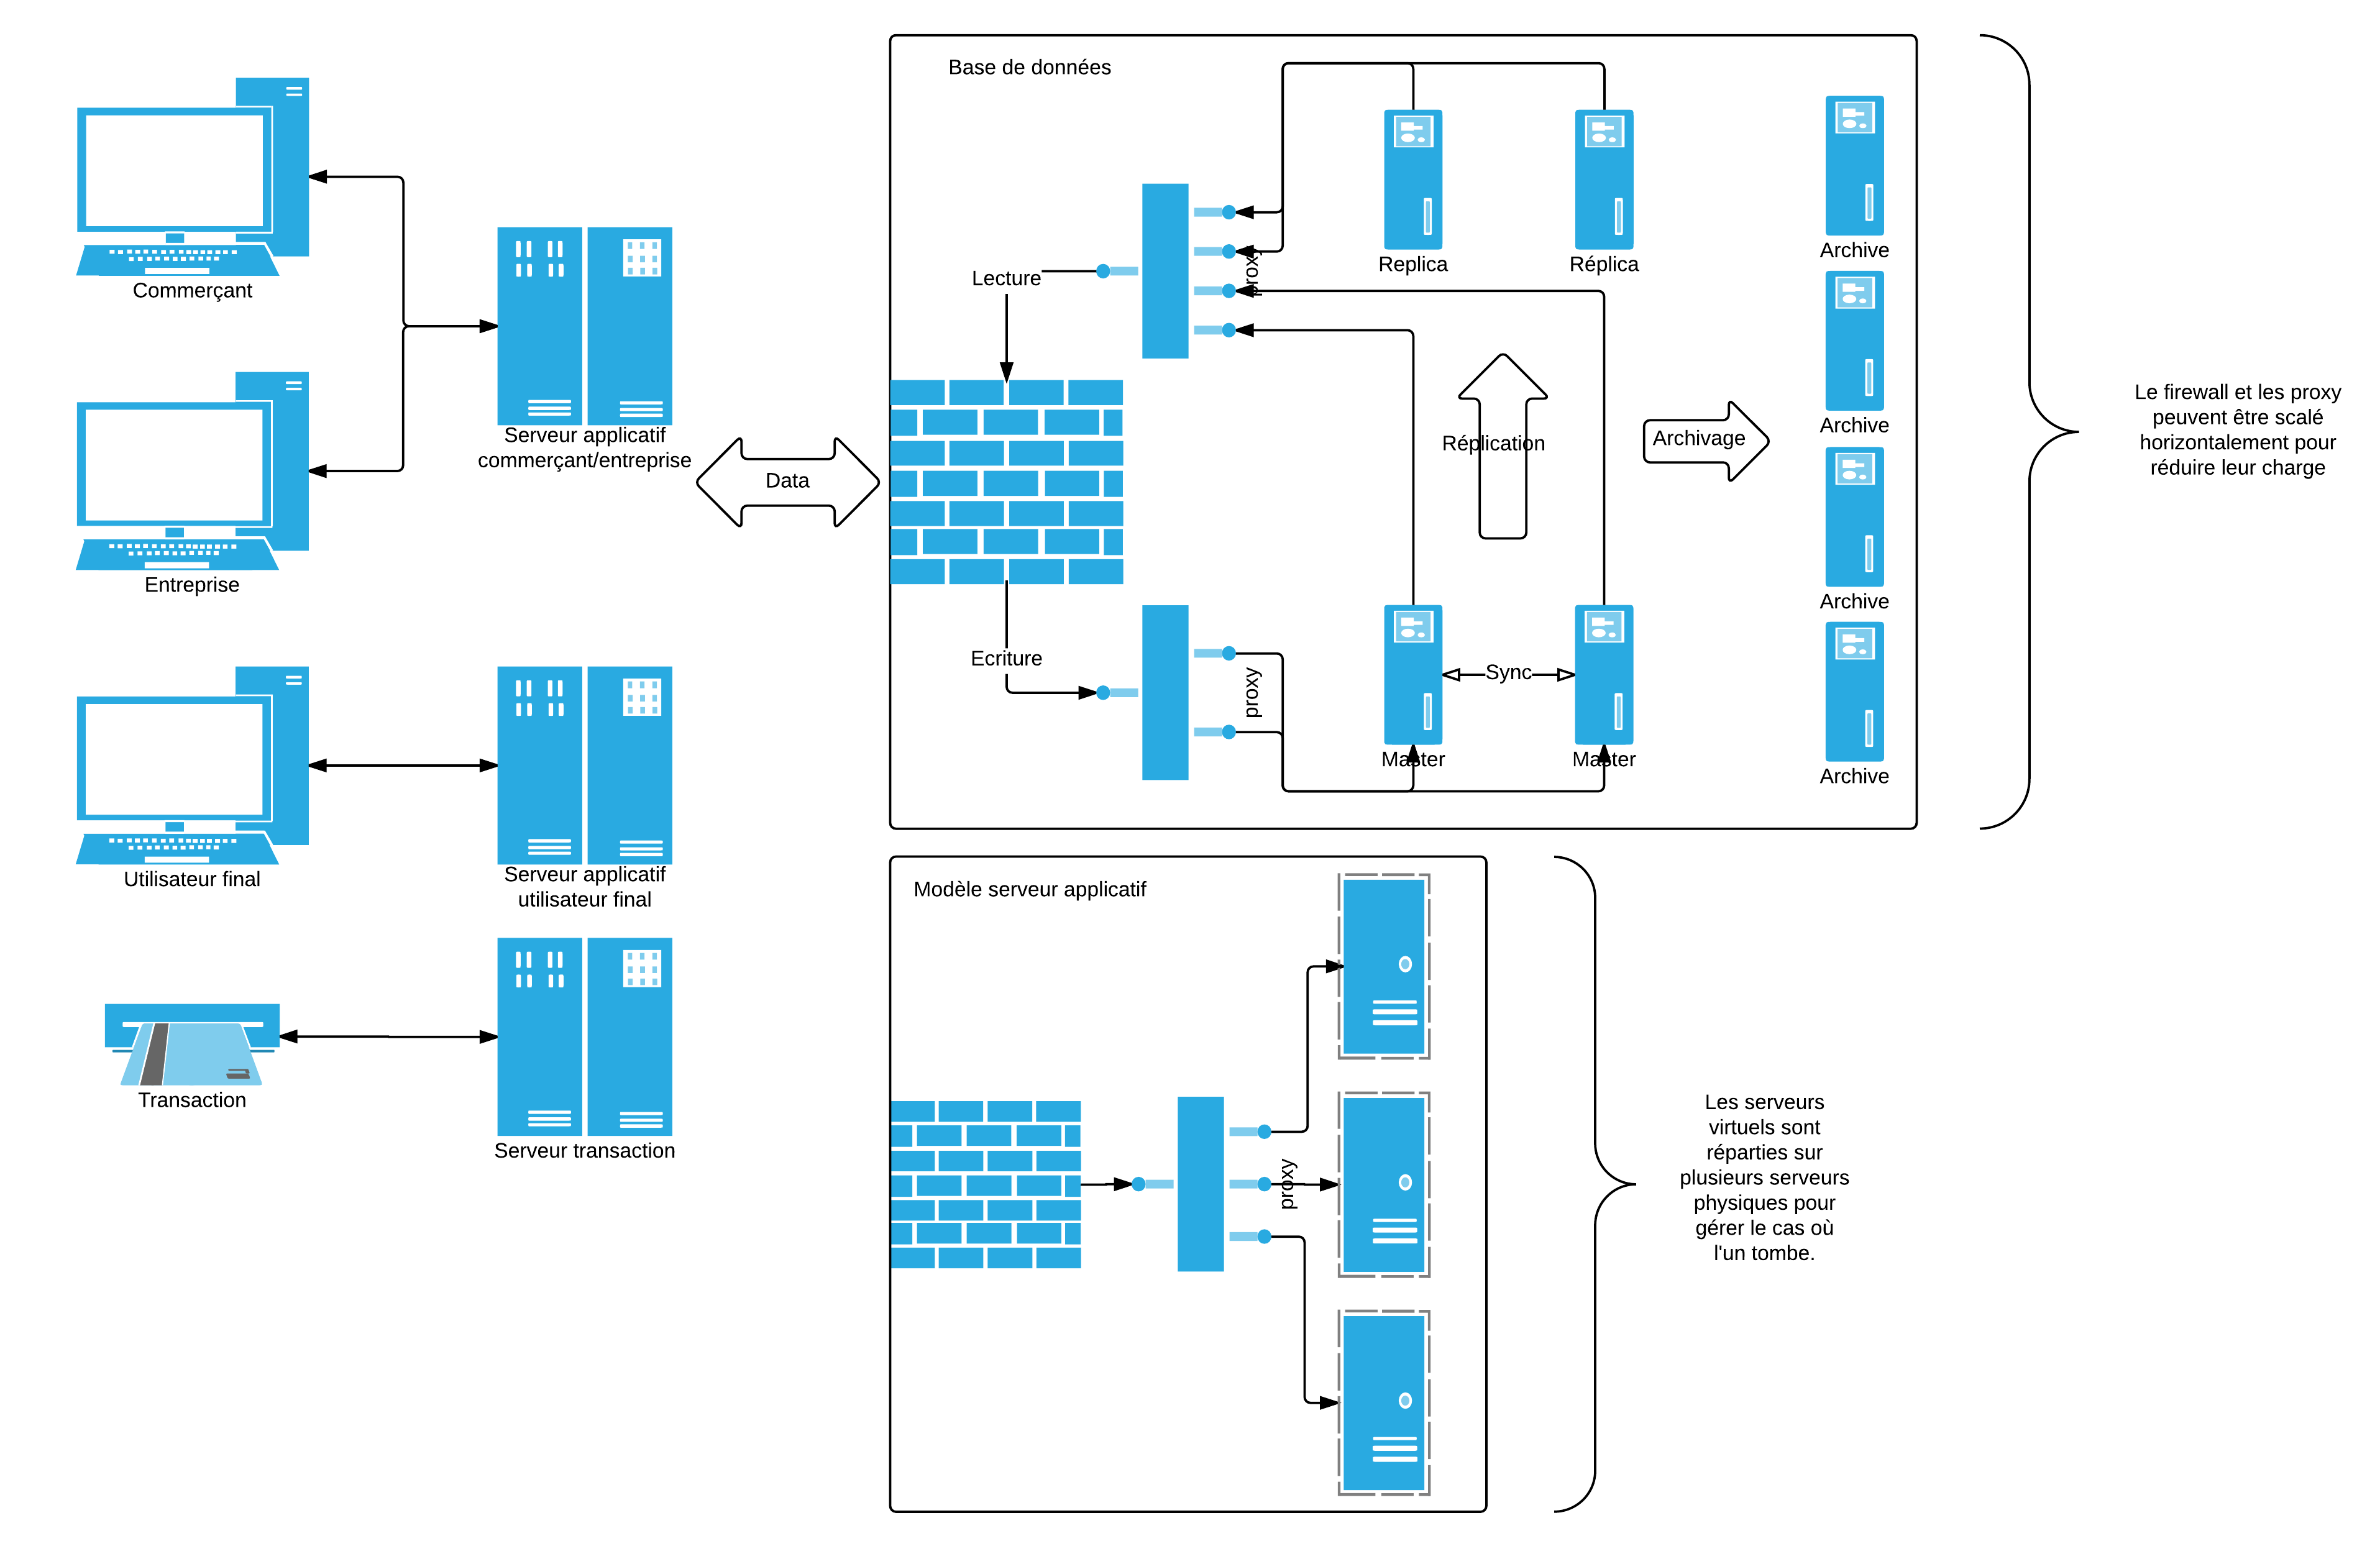
\includegraphics[width=0.7\paperheight]{network}
      \caption{Schéma général de l'architecture technique choisie}
      \label{fig:network}
  \end{figure}
\end{landscape}

\paragraph{Serveurs applicatifs}

L'accès aux serveurs applicatifs est gouverné par une couche \textbf{firewall}
et une couche \textbf{proxy}. La couche firewall est nécessaire pour gérer le
trafic indésirable (se référer à la section
\ref{subsec:securite-trafic} pour plus de détails). La couche proxy
permet de gérer le passage à l'échelle des serveurs applicatifs. \\

Le principe général du passage à l'échelle des serveurs applicatifs est basé
sur la duplication et synchronisation de plusieurs instances des serveurs
applicatifs, avec balance de charge sur ces dernières, régie par le proxy (se
référer à la section {\huge \textbf{TODO} } pour plus de détails).

\paragraph{Base de données}

L'accès au sous-système de base de données est régi par un firewall,
spécifiquement conçu pour le SGBD choisi. L'idée est de bloquer l'accès au
sous-système de base de données au monde extérieur, autorisant uniquement
l'accès au proxy servant à répartir les accès aux différentes bases de données
"maîtres". \\

De plus, un système de cache est configuré sur les serveurs de bases de données,
pour réduire la latence due à l'accès au sous-système de base de données, ainsi que
la charge qui lui est soumise.

\section{Dimensionnement}
\label{sec:Dimensionnement}

Bien que nos perspectives de développement varient grandement suivant l'échéance
considérée (Confer Business plan), on peut envisager un dimensionnement
des besoins immédiats en termes de charge supportée. \\

Notre stratégie marketing aggressive nous permet de nous positionner, dès notre
entrée sur le marché, en tant qu'acteurs majeurs du secteur, avec pas moins de
300 000 entreprises clientes, de toutes tailles, ce qui laisse présager aux
alentours de 6 millions de cartes à puce en circulation. \\

Ces cartes pourraient être utilisées sur l'une des 14 500 bornes de paiement mises
à disposition dans l'un des quelques 4 300 supermarchés et hypermarchés de zone
urbaine ou périurbaine équipés, ou encore dans un des quelques 50 000 restaurants
partenaires. \\

Ces infrastructures et ce modèle de déploiement rapide et massif nous laissent
espérer un volume de transactions quotidien important :

\begin{itemize}
    \item de l'ordre de 600 000 transactions quotidiennes dans les supermarchés,
    \item et 1 800 000 transactions dans les diverses enseignes de restauration.
\end{itemize}

Ces transactions seront bien évidemment concentrées sur quelques heures de pointe.
On peut attendre 60\% de la charge le midi, contre 30\% le soir et seulement 10\%
pour le reste de la journée. Le pic critique serait entre 12h20 et 12h40, où
presque 30\% des transactions quotidiennes sont attendues (soient quelques
720 000 transactions en seulement 20 minutes).

\section{Choix de la solution cloud}
\label{sec:choix-solution-cloud}

Chaque transaction pèse au plus 3 KB lors de sa validation. Le stockage,
une fois archivé, en est optimisé (sur le modèle du Bitcoin). \\

Lors du pic quotidien, 720 000 transactions sont attendues en l'espace de 20
minutes (1200 secondes), ce qui représente une moyenne de 600 transactions
par seconde (note : pour l'estimation de débit, nul besoin de lisser les
transactions sur leur durée. Ce calcul sera en revanche nécessaire lors
de l'estimation du volume de connexions simultanées). \\

Cela représente un besoin en débit de 1 800 KB/s en pointe. \\

Ces besoins en débit, plutôt modestes, nous permettent de nous diriger
vers une architecture fondée sur une forte virtualisation. \\

Pour assurer une meilleure QoS, nos efforts matériels ne seront pas concentrés
sur une seule machine, mais répartis sur au moins deux machines dans le cloud
(ce nombre pourra croître à mesure que grandiront nos besoins).

Nous avons opté pour une solution proposée par Amazon (gamme AWS), à savoir deux
serveurs Linux C3.4xlarge, chacun doté de 8 coeurs, 15GiB de RAM et 2 disques SSD
de 80GB chacun. Ces serveurs seront situés respectivement à Dublin et Francfort. \\

La faible volumétrie de stockage, à laquelle nous sommes contraints par les
enjeux budgétaires soulevés, sera compensée par une délégation de ce rôle à
des serveurs physiquement hébergés par nos soins.

\section{Passage à l'échelle (scaling)}
\label{sec:scaling}

\subsection{Scaling des serveurs applicatifs}
\label{subsec:scaling-applicatif}

Les serveurs applicatifs sont disposés sous forme de serveurs virtuelles
réparties sur plusieurs machines physiques. La charge importante de requête
peut être soutenu en plaçant en parallèle ces serveurs. Avant ceux-ci, un proxy
permet de distribuer les connexions des utilisateurs parmi eux. Cela garantie
d'avoir une charge uniforme sur l'ensemble des serveurs. \\

Dans le cas où cette charge est jugé trop importante ou que Aventix souhaite
augmenter le potentiels de l'application, d'autres serveurs virtuelles sont à
placer en parallèles derrière le proxy. \\

La machine possédant le proxy doit aussi pouvoir accepter une très forte charge
de connexion réseau. Ce dernier peut également être multiplié en parallèle afin
de contenir la demande croissante. \\

Cette remarque est également valable pour le firewall. \\

Les applications sont alors distribués parmi des blocs de serveurs applicatifs.
Nous avons choisi de placer les applications de gestion des commerçant et des
entreprises sur le même bloc de serveur. L'application de gestion des clients
et l'application de transaction ont chacun leur propre bloc de serveur. \\

Cette répartition permet de distribuer manuellement la charge sur différents
ensembles de machines. Egalement, cela rend les différentes applications
totalement indépendantes et une grave erreur sur l'une n'aura aucune
répercution sur les autres. \\

\subsection{Scaling des serveurs de bases de données}
\label{subsec:scaling-bdd}

L'ensemble du groupe servant de serveurs de bases de données est représenté par
un firewall, un proxy et un ensemble de serveur de données. \\

Le firewall et le proxy sont regroupés dans une même machine. Comme les
serveurs applicatifs, ces éléments permettent de garantir la sécurité et la
répartition de la charge sur l'ensemble des serveurs de base de données. \\

Les serveurs de base de données suivent un modèle de réplication multi-maître.
Plusieurs machines peuvent donc être placé en parallèle afin de supporter une
grande charge. \\

A l'instar des serveurs applicatifs, une croissance de l'ensemble de
l'application et donc de la charge globale est possible en rajoutant d'autres
instances de base de données. \\

Un archivage des données est effectué au fur et à mesure de l'exécution de
l'application après un certain temps fixé. Pour s'adapter à la quantité de
mémoire potentiellement importante à stocker lors d'un archivage, de nouveaux
serveurs de stockage sont à rajouter également au fur et à mesure. \\

\section{Sécurité}
\label{sec:securite}

\subsection{Sécurité d'infrastructure}
\label{subsec:securite-infrastructure}

En choisissant une solution cloud, la disponibilité de l'infrastructure est
garantie par le prestataire cloud, en l'occurence \textbf{Amazon AWS}. Le
système peut donc être considéré relativement sécurisé vis-à-vis des attaques
par déni de service (DoS simple), ou autre attaque d'infrastructure. \\

De plus, la disponibilité du système est dépendante de la disponibilité d'AWS,
en l'occurence celle-ci peut être assurée selon le prix de la prestation. Le
taux de panne de 0\% ne peut malheureusement pas l'être, du fait du nombre de
facteurs externes entrant en jeu. Cependant, un taux de 99\%, voire jusqu'à
99.95\% peut l'être par AWS (source: \url{http://aws.amazon.com/ec2/sla/}). \\

En passant par une solution cloud, le système est aussi protégé des attaques
physiques (coupure générale, attaque électromagnétique, etc...), mais encore
dépendant de l'infrastructure d'AWS. \\

Toutefois, une exception aux propositions demeure : le \textbf{sous-système de
base de données ne réside pas intégralement dans le cloud}. Ce problème n'est
pas d'une ampleur catastrophique, il faut noter qu'on est relativement bien
protégé des attaques DoS grâce au pare-feu conçu spécifiquement pour contrôler
l'accès et donc empêcher le trafic intempestif. \\

Malheureusement les attaques physiques peuvent atteindre le sous-système de
base de données, c'est la faiblesse majeure du système. Pour limiter davantage
la vulnérabilité physique du système, deux baies de serveurs en syncronisation
multi-master seront installées sur deux locaux différents (détaillé dans la
section {\huge \textbf{TODO}}.

\subsection{Sécurité du trafic}
\label{subsec:securite-trafic}

Le trafic indésirable correspond au trafic qui n'est pas directement lié à
l'utilisation normale du système. Il peut être utilisé comme attaque visant à
exploiter des failles d'autres services présents sur la VM, ou tout
simplement à réduire la disponibilité du système en multipliant les
accès (DoS). \\

EC2 met à disposition un firewall pour ses instances, ce qui permet de régler
son accès. Cependant, les VM étant installées à l'intérieur d'une instance,
elles doivent toutes être configurées séparément pour accepter uniquement le
trafic qui les concerne.

\paragraph{Fermeture maximale}

Un document relatant des conseils de sécurisation d'instance EC2, produit par
ce même service, est disponible à l'adresse suivante :
\url{http://aws.amazon.com/articles/1233/} (en date du \today). L'idée est
simplement de n'autoriser que le trafic qui est attendu, et par défaut de
bloquer toute connexion entrante ne correspondant pas à une règle spécifiée.

\paragraph{Chiffrement des messages}

La totalité des échanges de messages avec le système sera effectuée en
utilisant une authentification par clé. Il faudra par exemple acheter un
\textbf{certificat SSL} pour permettre l'utilisation du protocole HTTPS pour
accéder aux différentes applications web. Le dialogue avec les bornes sera
quant à lui chiffré par une méthode utilisant la cryptographie asymétrique (clé
publique).

\end{document}
